\documentclass[handout]{beamer}
%\documentclass[compress]{beamer}

%\documentclass{beamer}
\usepackage[T1]{fontenc}
\usepackage{pifont}
\usepackage{threeparttable}
\usepackage{subcaption}
\usepackage{tikz-qtree}
\usepackage{listings}
\usepackage[american]{babel}
\usepackage{csquotes}
\usepackage[style=apa, backend=biber]{biblatex}
\usepackage{tikz}
\usepackage{multicol}
\usepackage{booktabs}
\usepackage{graphicx}
\usepackage{neuralnetwork}
\usepackage{hyperref}
\usepackage{fancyvrb}

\usepackage{minted}
\definecolor{listingbg}{rgb}{0.87,0.93,1}
\setminted[python]{
breaklines,
linenos,
fontsize=\scriptsize,
frame=single,
xleftmargin=0pt}

\hypersetup{
    pdfborder={0 0 0},
    colorlinks=true,
}
\usetheme[block=fill,subsectionpage=progressbar,sectionpage=progressbar]{metropolis} 

\definecolor{Purple}{HTML}{911146}
\definecolor{Orange}{HTML}{CF4A30}

\setbeamercolor{alerted text}{fg=Orange}
\setbeamercolor{frametitle}{bg=Purple}

\setbeamercovered{still covered={\opaqueness<1->{5}},again covered={\opaqueness<1->{100}}}

\lstset{
    basicstyle=\scriptsize\ttfamily,
    columns=flexible,
    breaklines=true,
    numbers=left,
    %stepsize=1,
    numberstyle=\tiny,
    backgroundcolor=\color[rgb]{0.85,0.90,1}
}

\lstnewenvironment{lstlistingoutput}{\lstset{
        basicstyle=\footnotesize\ttfamily,
        columns=flexible,
        breaklines=true,
        numbers=left,
        %stepsize=1,
        numberstyle=\tiny,
        backgroundcolor=\color[rgb]{.7,.7,.7}}}{}


\lstnewenvironment{lstlistingoutputtiny}{\lstset{
        basicstyle=\tiny\ttfamily,
        columns=flexible,
        breaklines=true,
        numbers=left,
        %stepsize=1,
        numberstyle=\tiny,
        backgroundcolor=\color[rgb]{.7,.7,.7}}}{}

\renewcommand*{\bibfont}{\tiny}

\makeatletter
\setbeamertemplate{headline}{%
    \begin{beamercolorbox}[colsep=1.5pt]{upper separation line head}
    \end{beamercolorbox}
    \begin{beamercolorbox}{section in head/foot}
        \vskip2pt\insertnavigation{\paperwidth}\vskip2pt
    \end{beamercolorbox}%
    \begin{beamercolorbox}[colsep=1.5pt]{lower separation line head}
    \end{beamercolorbox}
}
\makeatother

\newcommand{\question}[1]{
    \begin{frame}[plain]
        \begin{columns}
            \column{.4\textwidth}
            \makebox[\columnwidth]{
                
\includegraphics[width=\columnwidth,height=\paperheight,keepaspectratio]{mannetje.png}}
            \column{.6\textwidth}
            \large
            \textcolor{orange}{\textbf{\emph{#1}}}
        \end{columns}
    \end{frame}}

\newcommand{\instruction}[1]{\emph{\textcolor{gray}{[#1]}}}

\addbibresource{resources/literature.bib}
\graphicspath{{resources/pictures/}}

\title[Computational Communication Science 2]{\textbf{Computational Communication Science 2} \\[0.3cm] 
\large{Week 1}\\[0.2cm]
\emph{Introduction \& Lift Off}}

\author[Anne Kroon, Saurabh Khanna]{\textbf{Anne Kroon} \\ \footnotesize{a.c.kroon@uva.nl} \\[0.2cm] 
\textbf{Saurabh Khanna} \\ \footnotesize{s.khanna@uva.nl}}

\date[\today]{March 31, 2025}

\institute[Digital Society Minor, UvA]{\small Digital Society Minor \\ University of Amsterdam}

\begin{document}

\begin{frame}{}
	\titlepage
\end{frame}
	
\begin{frame}{Today}
	\tableofcontents
\end{frame}

\section[The people]{Introducing\ldots the people}

\begin{frame}{Introducing\ldots \huge{Saurabh}} 
	\begin{columns}
		\column{.3\textwidth}
		\makebox[\columnwidth]{
			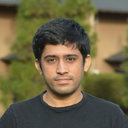
\includegraphics[width=\columnwidth,height=\paperheight,keepaspectratio]{../pictures/Saurabh-Khanna-2.png}}
		\column{.7\textwidth}
		dr. Saurabh Khanna \\
		Assistant Professor, Youth \& Media Entertainment 
		\begin{itemize}
			\item Studying the limits of human knowledge in an increasingly digitized world using
			\begin{itemize}
				\item Computational methods 
			\end{itemize}
		\end{itemize}
		\textbar s.khanna@uva.nl \textbar \url{https://www.uva.nl/en/profile/k/h/s.khanna/s.khanna.html} 
	\end{columns}
\end{frame}

\begin{frame}{Introducing\ldots \huge{Anne}} 
	\begin{columns}[] \column{.3\textwidth} \makebox[\columnwidth]{ 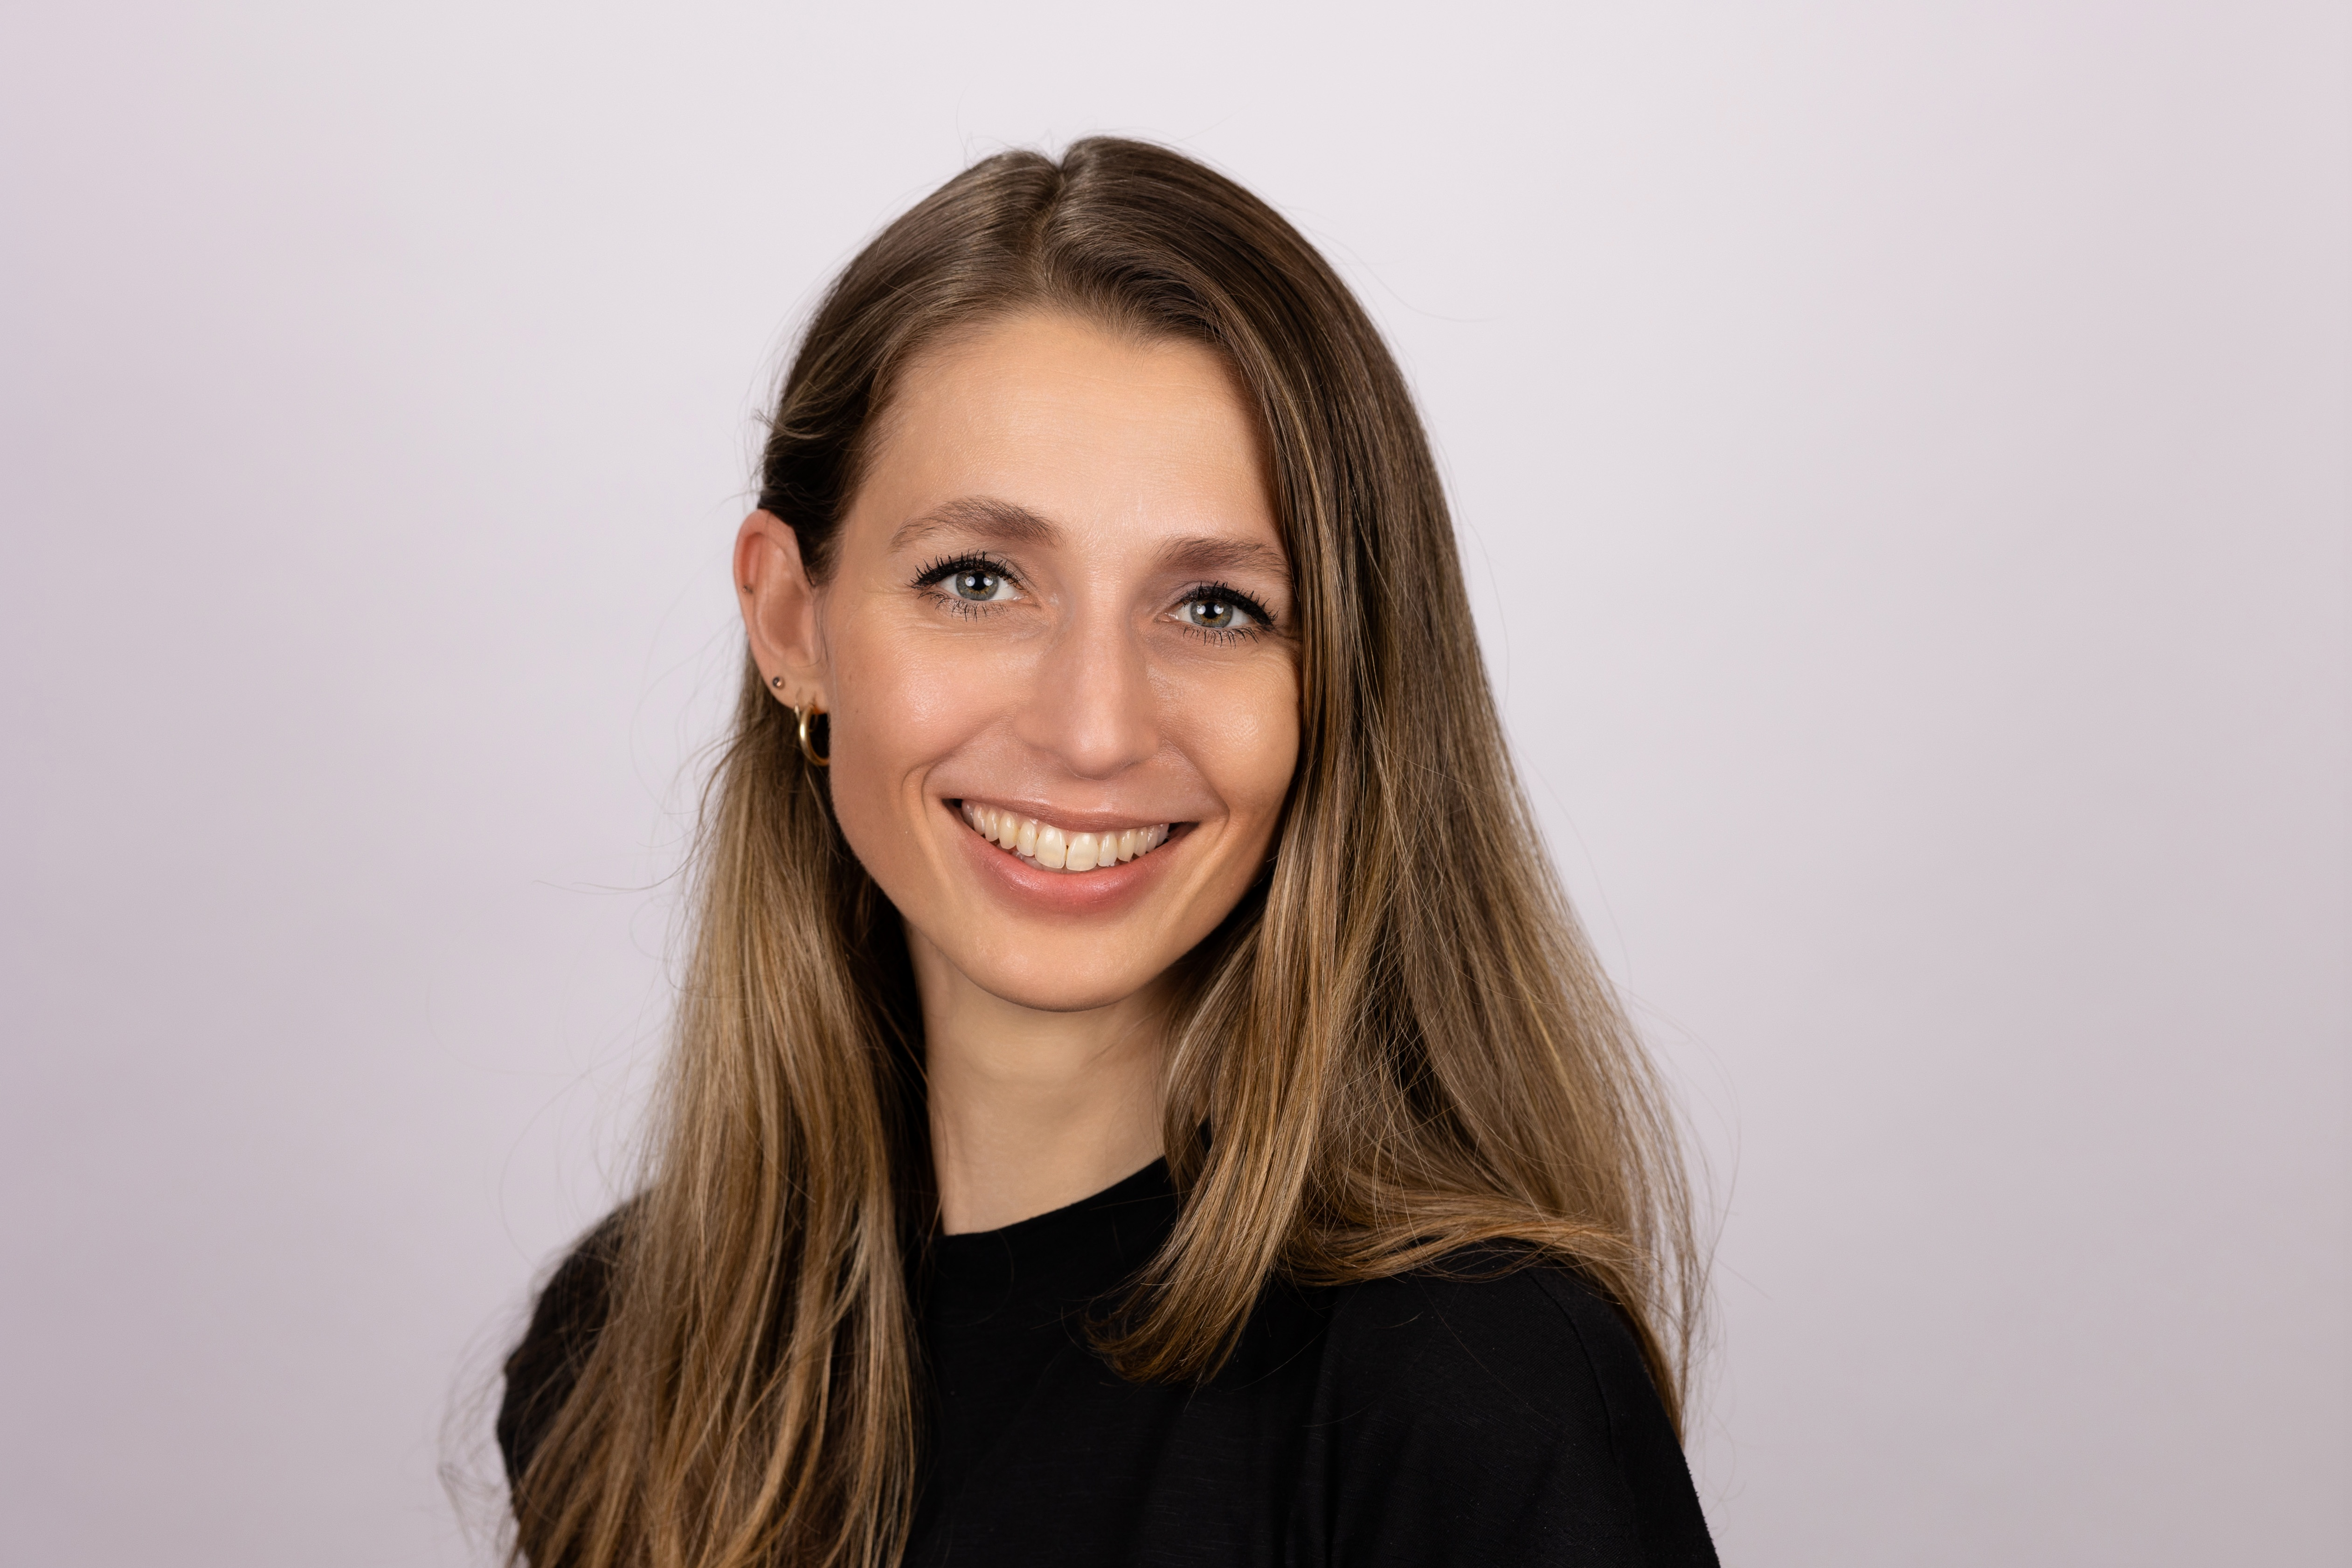
\includegraphics[width=\columnwidth,height=\paperheight,keepaspectratio]{../pictures/anne.jpg}} \column{.7\textwidth} dr. Anne Kroon \\ 
		Associate Professor Communication, Organizations \& Society
		\begin{itemize} 
			\item Research focus on biased AI in recruitment, and media bias regarding minorities
			\item Text analysis using automated approaches, word embeddings
		\end{itemize} @annekroon \textbar a.c.kroon@uva.nl  \textbar \\ \url{http://www.uva.nl/profiel/k/r/a.c.kroon/a.c.kroon.html} 
	\end{columns} 
\end{frame}

\section[The course]{Introducing\ldots the course}

\begin{frame}{About CCS-2} 
What is CCS-2?
	\begin{itemize}
		\item Next step after CCS-1 
		\item Learn how to use what you learned in CCS-1 for research
		\item Expand on what you learned in CCS-1
		\begin{itemize}
			\item Learn computational techniques (e.g. data vectorization, machine learning)
			\item Learn how to use these techniques for research (e.g., automated content analysis)
		\end{itemize}
		\item By the end of the course, you'll be prepared for the \emph{Research Project}
	\end{itemize}
	
\end{frame}

\begin{frame}{About CCS-2}
	\begin{center}
		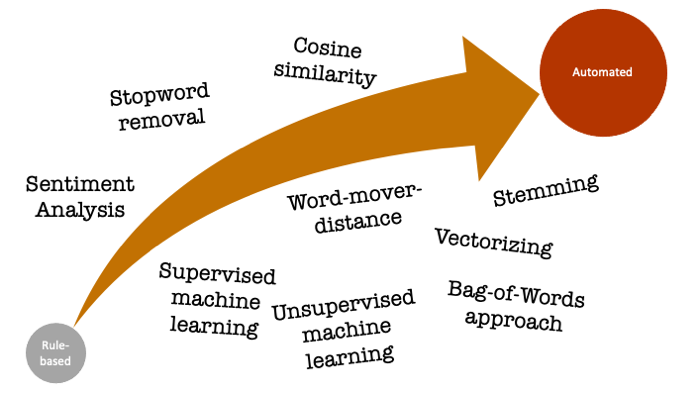
\includegraphics[width=\linewidth,height=\textheight,keepaspectratio]{../pictures/Roadmap_terms.png} 
	\end{center}
\end{frame}


\begin{frame}{About CCS-2} 

What will we do in this course?	
	\begin{itemize}[<+->]
		\item We discuss techniques in the lectures (Mondays)
		\item We practice with techniques in the tutorials (Tuesdays)
		\item Graded assignments to master the techniques:
		\begin{itemize}
			\item Regular multiple choice questions (\(20\%\)) about the readings and techniques that we discuss
			\begin{itemize}
				\item 4 questions, in week 1, 2, 3, 7 and 8. 
				\item \emph{total of 20 questions. 16 correct answers = full marks}
			\end{itemize}
			\item Group assignment: Get more experienced with the techniques and build a \emph{basic} recommender system
			\begin{itemize}
				\item Written report and code assignment (\(20\%\))
                    \item Presentation -- week 6 (\(10\%\))
			\end{itemize}
			\item In-class exam on May 27th (\(50\%\)): at the end of the course so you can show off what you learned
		\end{itemize}
		\item We provide structure through the meetings and assignments, you do the (home-)work
	\end{itemize}
	
\end{frame}

\begin{frame}{About CCS-2} 
	
Course set-up:
\begin{itemize}[<+->]
	\item \emph{Lectures}: Introduction to techniques used in computational communication science
	\item \emph{Tutorial meetings}: Lab sessions to learn how to work with these techniques
	\begin{itemize}
		\item Possibility to ask questions about your code
	\end{itemize}
\end{itemize}

\end{frame}

\begin{frame} 
	All course materials can be found at\ldots \\
	~~~~~~~~\url{https://github.com/uva-cw-ccs2/2425s2}
\end{frame}

\begin{frame}{About CCS-2} 
How to stay informed and where to find all the materials? Regularly check:	
	\begin{itemize}
		\item The course Canvas page
		\item Your email
		\item The course Github page
	\end{itemize}
In addition, make sure that you read the course manual so that you know all the ins and outs of this course!
\end{frame}


\begin{frame}{Ready? Set? Go!} 
	
	Without further ado\dots
	
	\dots let's get started!
	
\end{frame}

\section{Text as data}

\begin{frame}{Text as data}
	CCS-1: You learned how to...
		\begin{itemize}
		\item Work with Python, for example, you:
		\begin{itemize}
			\item Store text in json-files, csv-files etc.
			\item Difference between a dict, a list, a string etc.
			\item Work with data (e.g., creating a loop)
		\end{itemize}
	\end{itemize}
	\end{frame}

\begin{frame}{Text as data: Analyzing text as a goal}
	Studying text can teach us a lot about human behavior:
	\begin{itemize}[<+->]
	\item \dots to study the content cancer-related online platforms (e.g., \cite{sanders_different_2020})
	\begin{itemize}
	\item what \emph{topics} are being discussed on expert and peer-generated platforms?
	\end{itemize}
	\item \dots does content differ between online and print news? (e.g., \cite{burggraaff_through_2020})
	\begin{itemize}
	\item E.g., online, journalists are more likely to publish \emph{follow-up} articles.
	\end{itemize}
	\end{itemize}
\end{frame}
	
\begin{frame}{Text as data: Analyzing text as a means}
Studying text can give us information we can use to answer broader questions: 
\begin{itemize}[<+->]
	\item \dots analyze textual information about movies from IMDB to learn about the representation of women in movies (e.g.,\cite{poma-murialdo_gender_2019} )
	\item \dots automatically distinguish between reliable and unreliable online information about vaccines 
	by investigating what characterizes reliable and unreliable texts (e.g.,\cite{meppelink_reliable_2021})
\end{itemize}
\end{frame}

\begin{frame}{Computational communication science}

    \begin{columns}[T]
        \begin{column}{0.6\textwidth}
            \begin{block}{New opportunities}
                Gaining insights from large-scale digital data.
            \end{block}

            \vspace{0.2cm}
            \begin{itemize}
                \item \textbf{Digital traces:} Social media, news, and archives.
                \item \textbf{New tools:} Network and sentiment analysis, text mining.
                \item \textbf{Big data:} Analyzing complex datasets at scale.
            \end{itemize}
        \end{column}

        \begin{column}{0.4\textwidth}
            
\includegraphics[width=0.85\textwidth]{../pictures/doge-big-data-meme.jpg}
        \end{column}
    \end{columns}

    \vspace{0.3cm}
    \begin{block}{Why it matters:}
        Real behavior \textbullet\ Natural contexts \textbullet\ Hidden patterns \textbullet\ Collaboration.
    \end{block}

\end{frame}


\begin{frame}{Challenges in computational research}

    \begin{block}{Key challenges}
        \begin{itemize}
            \item \textbf{Data access:} Ensuring open and reproducible datasets.
            \item \textbf{Data validity:} Addressing biases and representativeness.
            \item \textbf{Measurement:} Evaluating the accuracy of automated analyses.
            \item \textbf{Ethics:} Protecting privacy and ensuring responsible data use.
        \end{itemize}
    \end{block}

    \vspace{0.5cm}
    \begin{block}{Takeaway}
        Blending traditional and computational approaches strengthens theory-driven research.
    \end{block}

    \vspace{0.3cm}
    \small \textbf{Reference:} \cite{vanAtteveldt2018}

\end{frame}


\begin{frame}{Text as data: natural language processing (NLP)}

    \begin{columns}[T] % Align text and image in columns
        \begin{column}{0.6\textwidth}
            \begin{block}{What is NLP?}
                Natural language processing (NLP) is a branch of computer science—specifically artificial intelligence (AI)—that enables computers to understand and interpret human language. 
            \end{block}
            \vspace{0.3cm}
            \small{\textit{(IBM, 2020)}}
        \end{column}

        \begin{column}{0.2\textwidth}
            \vspace{0.5cm}
            
\includegraphics[width=0.9\textwidth]{../pictures/sprinkle-it-in.jpg}
        \end{column}
    \end{columns}

    \vspace{0.4cm}

    \begin{block}{Want to know more?}
        Explore how NLP is reshaping data analysis in this TED Talk: \\
        \small{\url{https://www.ted.com/talks/jean_baptiste_michel_erez_lieberman_aiden_what_we_learned_from_5_million_books}}
    \end{block}

\end{frame}



\section{The Toolkit}

\subsection{Bottom-up vs. Top-down}

\begin{frame}[standout]
Automated content analysis can follow two main approaches:
\begin{itemize}
\item \textcolor{red}{Bottom-up}: Inductive, explorative, based on pattern recognition.
\item \textcolor{red}{Top-down}: Deductive, guided by pre-defined rules and categories.
\end{itemize}
Or, it can lie somewhere in between.
\end{frame}

\begin{frame}{The CCS Toolbox in Practice}
\centering
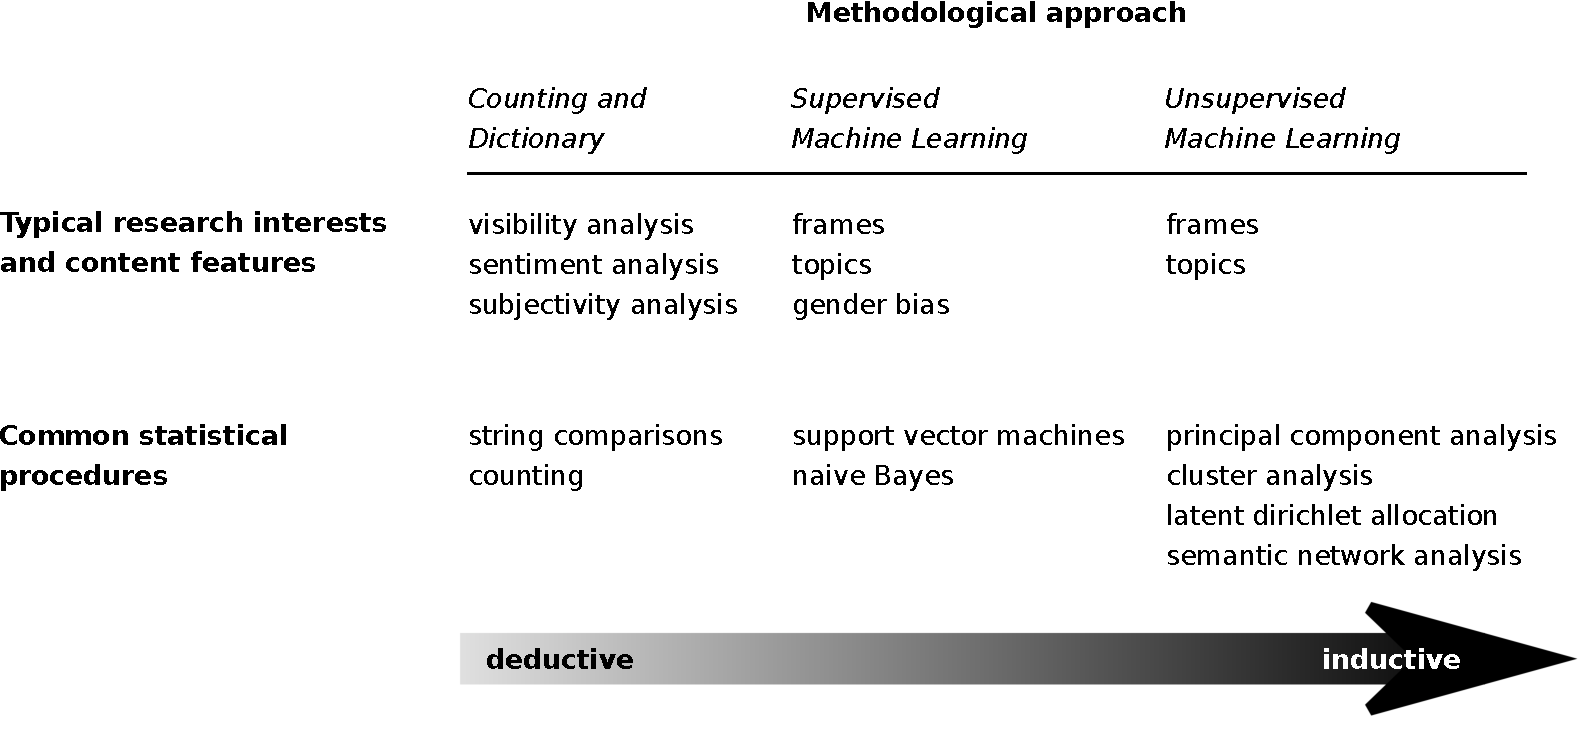
\includegraphics[width=0.9\columnwidth]{../pictures/boumanstrilling2016}

\vspace{0.5cm}
\small{Source: \cite{Boumans2016}}
\end{frame}

\begin{frame}{Understanding the approaches}
\begin{columns}
\column{0.5\textwidth}
\begin{block}{\textbf{Bottom-up}}
\begin{itemize}
\item Identify frequent words or patterns.
\item Explore word co-occurrence: \emph{Which words appear together?}
\end{itemize}
\textbf{Key idea:} We \emph{don't} specify what to look for in advance.
\end{block}

\column{0.5\textwidth}
\begin{block}{\textbf{Top-down}}
\begin{itemize}
\item Track occurrences of pre-defined words.
\item Identify specific patterns of interest.
\end{itemize}
\textbf{Key idea:} We \emph{do} specify what to look for in advance.
\end{block}
\end{columns}
\end{frame}

\begin{frame}{Research example of bottom-up approach (data-driven)}

    \begin{block}{Word co-occurrence graphs in disease surveillance}
        \begin{itemize}
            \item Analyzes co-occurrence of words to identify patterns in disease reporting.
            \item Useful for detecting emerging trends without predefined categories.
        \end{itemize}
        \begin{center}
            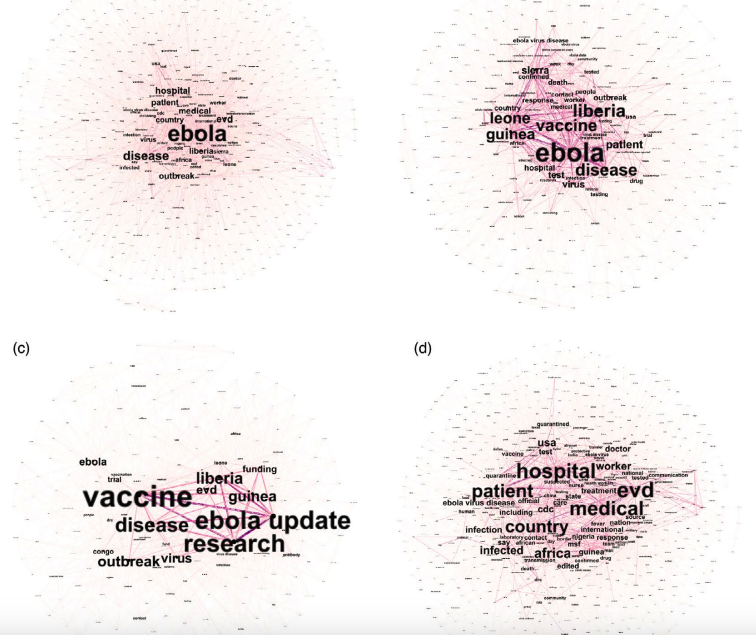
\includegraphics[width=0.4\linewidth]{../pictures/wordcloud.png}
            \small \cite{you2021using} % Subtle citation
        \end{center}
    \end{block}

\end{frame}


\begin{frame}{Research example of top-down approach (theory-driven)}
    \begin{block}{Sentiment analysis using LIWC}
        \begin{itemize}
            \item LIWC is a widely applied (commercial and closed) software tool.
            \item Counts occurrences of predefined terms (e.g., psychological and linguistic categories).
            \item Guided by theoretical frameworks; useful for hypothesis testing and interpreting psychological states—but does it work?
        \end{itemize}
    \end{block}
    \vspace{0.5cm}
    \small \cite{tausczik2010psychological} % Subtle citation
\end{frame}


\begin{frame}{LIWC application in online support groups}

    \begin{itemize}
        \item LIWC was used to analyze language in online support groups for breast cancer patients \cite{shim2011does}.
        \item It categorizes words into emotional and cognitive dimensions (e.g., insight, positive/negative emotion).
        \item The study found that insightful disclosure improved emotional and functional well-being by reducing breast cancer concerns.
    \end{itemize}

    \begin{center}
        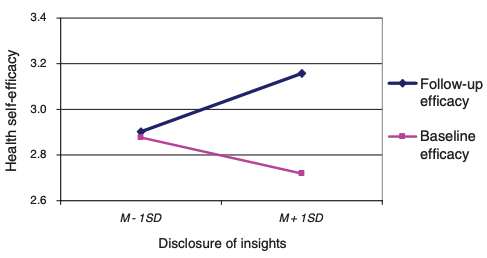
\includegraphics[width=0.8\linewidth]{../pictures/LIWC.png}
    \end{center}

\end{frame}

\begin{frame}{Linking bottom-up and top-down approaches}

    \begin{itemize}
        \item Both approaches complement each other in computational communication science \cite{vanAtteveldt2018}.
        
        \item \textbf{Bottom-up:} Ideal for exploring data and discovering unknown patterns.
        
        \item \textbf{Top-down:} Useful for testing established theories and measuring specific constructs.
        
        \item \textbf{Why combine them?} It enables a more comprehensive analysis—uncovering new insights while validating theoretical frameworks.
    \end{itemize}

    \vspace{0.5cm}

\end{frame}




\subsection{Hands-on examples}

\begin{frame}[fragile]{A simple bottom-up approach}
\textbf{Goal:} Identify frequent words in a text corpus.

\begin{minted}[fontsize=\tiny, frame=single]{python}
from collections import Counter
texts = ["Communication in the Digital Society is very very complex", "I like to study it"]
bottom_up = []
for t in texts:
    bottom_up.append(Counter(t.lower().split()).most_common(3))
print(bottom_up)
\end{minted}

\pause

This produces:

\begin{minted}[fontsize=\tiny, frame=single]{text}
[('very', 2), ('communication', 1), ('in', 1)]
[('i', 1), ('like', 1), ('to', 1)]
\end{minted}

\pause
\textbf{Equivalent with list comprehension:}

\begin{minted}[fontsize=\tiny, frame=single]{python}
bottom_up = [Counter(t.lower().split()).most_common(3) for t in texts]
\end{minted}

\vspace{0.2cm}
\textcolor{red}{\footnotesize{\emph{Tip: List comprehensions save space and improve speed!}}}
\end{frame}

\begin{frame}[fragile]{A Simple Top-down Approach}
\textbf{Goal:} Count specific word occurrences.

\begin{minted}[fontsize=\tiny, frame=single]{python}
texts = ["Communication in the Digital Society is complex", "I like to study it"]
features = ["communication", "digital", "study"]

top_down = []
for t in texts:
    counts = [t.lower().count(f) for f in features]
    top_down.append(counts)
print(top_down)
\end{minted}

\pause
This produces:

\begin{minted}[fontsize=\tiny, frame=single]{text}
[[1, 1, 0], [0, 0, 1]]
\end{minted}

\pause
\textbf{Equivalent with list comprehension:}

\begin{minted}[fontsize=\tiny, frame=single]{python}
top_down = [[t.lower().count(f) for f in features] for t in texts]
\end{minted}

\vspace{0.2cm}
\textcolor{red}{\footnotesize{\emph{Tip: Store results as lists for further analysis!}}}
\end{frame}


\question{When would you use which approach?}

\begin{frame}{Some considerations}
	\begin{itemize}[<+->]
		\item Both can have a place in your workflow (e.g., bottom-up as first exploratory step)
		\item You have a clear theoretical expectation? Bottom-up makes little sense.
		\item But in any case: you need to transform your text into something ``countable''.
	\end{itemize}
\end{frame}

\section{Preprocessing}

\begin{frame}
	\begin{block}{Preprocessing in NLP}
		\begin{itemize}	
	\item Text preprocessing in \emph{Natural Language Processing}. 
	\item Typical step to get textual data into a more structured format for subsequent analyses
	\item These steps will come back in the upcoming weeks when we discuss bottom-up and top-down techniques
		\end{itemize}
\end{block}
\end{frame}

\begin{frame}{Typical preprocessing steps}
	\begin{block}{Preprocessing steps}
		\begin{description}
			\item [\emph{tokenization}] How do we (best) split a sentence into tokens (terms, words)?
			\item [\emph{pruning}] How can we remove unneccessary words/ punctuation?
			\item [\emph{lemmatization and stemming}] How can we make sure that slight variations of the same word are not counted differently?
			\item [\emph{ngrams}] Neighbouring terms
		\end{description}
	\end{block}
\end{frame}

\begin{frame}[fragile]{Simple string methods}
	\begin{block}{Slicing}
		\texttt{mystring[2:5]} to get the characters with indices 2,3,4
	\end{block}
	\begin{block}{String methods}
		\begin{itemize}
			\item \texttt{.lower()} returns lowercased string
			\item \texttt{.strip()} returns string without whitespace at beginning and end
			\item \texttt{.find("bla")} returns index of position of substring ``bla'' or -1 if not found
			\item \texttt{.replace("a","b")} returns string where "a" is replaced by "b"
			\item \texttt{.count("bla")} counts how often substring ``bla'' occurs
		\end{itemize}
		Use tab completion for more!
	\end{block}
\end{frame}

%\subsection*{Tokenization}

\begin{frame}[fragile]{OK, good enough, perfect?}
	\begin{block}{.split()}
		\begin{itemize}
			\item space $\rightarrow$ new word
			\item no further processing whatsoever
			\item thus, only works well if we do a preprocessing outselves (e.g., remove punctuation)
		\end{itemize}
	\end{block}
\pause
\begin{minted}[%
	breaklines,
	linenos,
	fontsize=\scriptsize,
	frame=single,
	xleftmargin=0pt,]
	{python}
docs = ["This is a text",  "I haven't seen John's derring-do. Second sentence!"]
tokens = [d.split() for d in docs]
\end{minted}
	
\begin{minted}[%
	fontsize=\scriptsize,]
	{python}
[['This', 'is', 'a', 'text'], ['I', "haven't", 'seen', "John's", 
'derring-do.', 'Second', 'sentence!']]
\end{minted}
\end{frame}

\begin{frame}[fragile]{OK, good enough, perfect?}
	\begin{block}{Tokenizers from the NLTK package}
		\begin{itemize}
			\item multiple improved tokenizers that can be used instead of .split()
			\item e.g., Treebank tokenizer:
			\begin{itemize}
				\item split standard contractions ("don't")
				\item deals with punctuation
			\end{itemize}			
		\end{itemize}
	\end{block}
\pause
\begin{minted}[%
	breaklines,
	linenos,
	fontsize=\scriptsize,
	frame=single,
	xleftmargin=0pt,]
	{python}
from nltk.tokenize import TreebankWordTokenizer
tokens = [TreebankWordTokenizer().tokenize(d) for d in docs]
\end{minted}
\pause
\begin{minted}[%
breaklines,
fontsize=\scriptsize]
{python}
[['This', 'is', 'a', 'text'],  ['I', 'have', "n't", 'seen', 'John', "'s", 'derring-do.', 'Second', 'sentence', '!']]
\end{minted}
\tiny{Notice the failure to split the \texttt{.} at the end of the first sentence in the second doc. That's because \texttt{TreebankWordTokenizer} expects \emph{sentences} as input. See book for a solution.\\}
\end{frame}

%\subsection*{Stopword and punctuation removal}

\begin{frame}
	\textbf{Stopword removal} \\
	\vspace{1cm}
	\begin{itemize}
		\item <2->{\emph{The logic of the algorithm is very much related to the one of a simple sentiment analysis!}}
	\end{itemize}
\end{frame}

\begin{frame}{Stopword removal}
	\begin{block}{What are stopwords?}
		\begin{itemize}
			\item Very frequent words with little inherent meaning
			\item \texttt{the, a, he, she, \ldots}
			\item context-dependent: if you are interested in gender, \texttt{he} and \texttt{she} are no stopwords. 
			\item Many existing lists as basis
		\end{itemize}
	\end{block}
	
\end{frame}

\begin{frame}{Stopword removal: What and why?}
	\begin{block}{Why remove stopwords?}
		\begin{itemize}
			\item If we want to identify key terms (e.g., by means of a word count), we are not interested in them
			\item If we want to calculate document similarity, it might be inflated
			\item If we want to make a word co-occurance graph, irrelevant information will dominate the picture
		\end{itemize}
	\end{block}
\end{frame}

\begin{frame}[fragile]{Stopword removal}
\begin{minted}[%
	breaklines,
	linenos,
	fontsize=\scriptsize,
	frame=single,
	xleftmargin=0pt,]
	{python}
from nltk.corpus import stopwords
mystopwords = stopwords.words("english")
mystopwords.extend(["test", "this"])

tokens_without_stopwords = [[word for word in doc if word.lower() not in mystopwords] for doc in tokens]
\end{minted}
\begin{minted}[%
fontsize=\scriptsize,]
{python}
[['text'], ["n't", 'seen', 'John', 'derring-do.', 'Second', 'sentence', '!']]
\end{minted}
	
\begin{alertblock}{You can do more!}
		\tiny{For instance, you could add an \texttt{or} statement to also exclude punctuation.}
\end{alertblock}
	
\end{frame}

\begin{frame}[fragile]{Removing punctuation}
\begin{minted}[%
	breaklines,
	linenos,
	fontsize=\scriptsize,
	frame=single,
	xleftmargin=0pt,]
	{python}
from nltk.tokenize import RegexpTokenizer
tokenizer = RegexpTokenizer(r'\w+')
tokenizer.tokenize("Hi students, what's up!")
\end{minted}
\pause
\begin{minted}[%
	fontsize=\scriptsize,]
	{python}
['Hi', 'students', 'what', 's', 'up']
\end{minted}	
\end{frame}

%\subsection*{Stemming and lemmatization}


\begin{frame}{Tuesday April 1}
	\begin{block}{Tutorial meeting tomorrow}
		\begin{itemize}
                \item \emph{FIRST 4 MC QUESTIONS!}
			\item Start to practice with pre-processing techniques yourself
			\item Try the code in these slides at home. Make sure you can follow along.
			\item Use the tutorial meetings to discuss your questions.
		\end{itemize}
	\end{block}
\end{frame}

\begin{frame}{Practice is key!}
    \centering
    
\includegraphics[width=0.8\textwidth,height=0.8\textheight,keepaspectratio]{python_running.jpeg}
    %\footnote{https://towardsdatascience.com/what-is-cosine-similarity-how-to-compare-text-and-images-in-python-d2bb6e411ef0}
\end{frame}


\begin{frame}{Thank you!!}
	\begin{block}{Thank you for your attention!}
		\begin{itemize}
			\item Questions? Comments?
		\end{itemize}
	\end{block}
\end{frame}

\begin{frame}[t,allowframebreaks]
	\frametitle{References}
	\printbibliography
\end{frame}

\end{document}